\section{\name Prototype Implementation}
\label{sec:prototype}


\begin{figure}[t]
	\begin{center}
		\begin{subfigure}{0.4\textwidth}
		\centering
			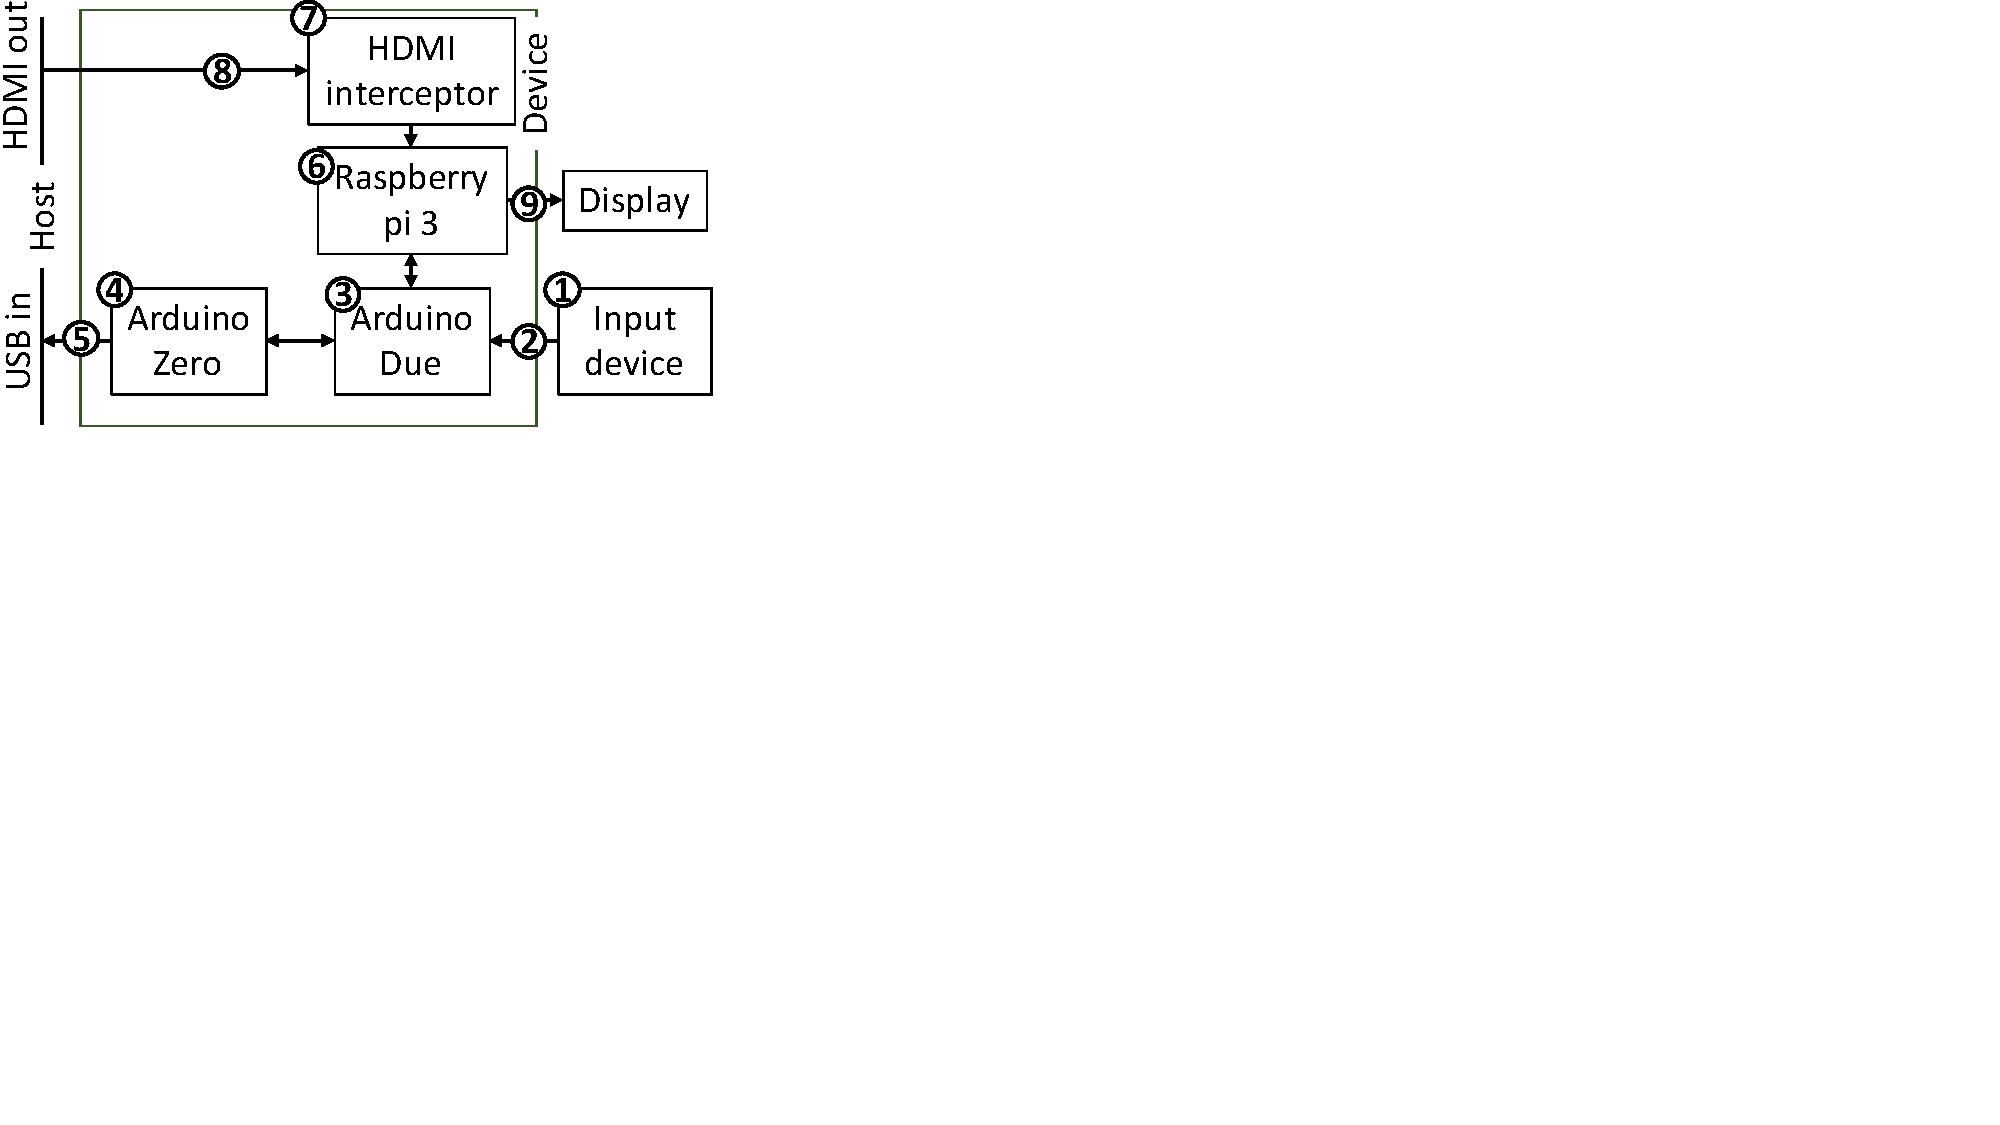
\includegraphics[trim={0 12cm 21.7cm 0}, clip, scale=0.5]{setUpBlock.pdf}
			\caption{The figure shows the basic components and connections between them in our \name prototype.}
			\label{fig:prototypeArch}	
		\end{subfigure}
	\end{center}
	
	%\vspace{1em} 
	
	\begin{center}
		\begin{subfigure}{0.4\textwidth}
		\centering
		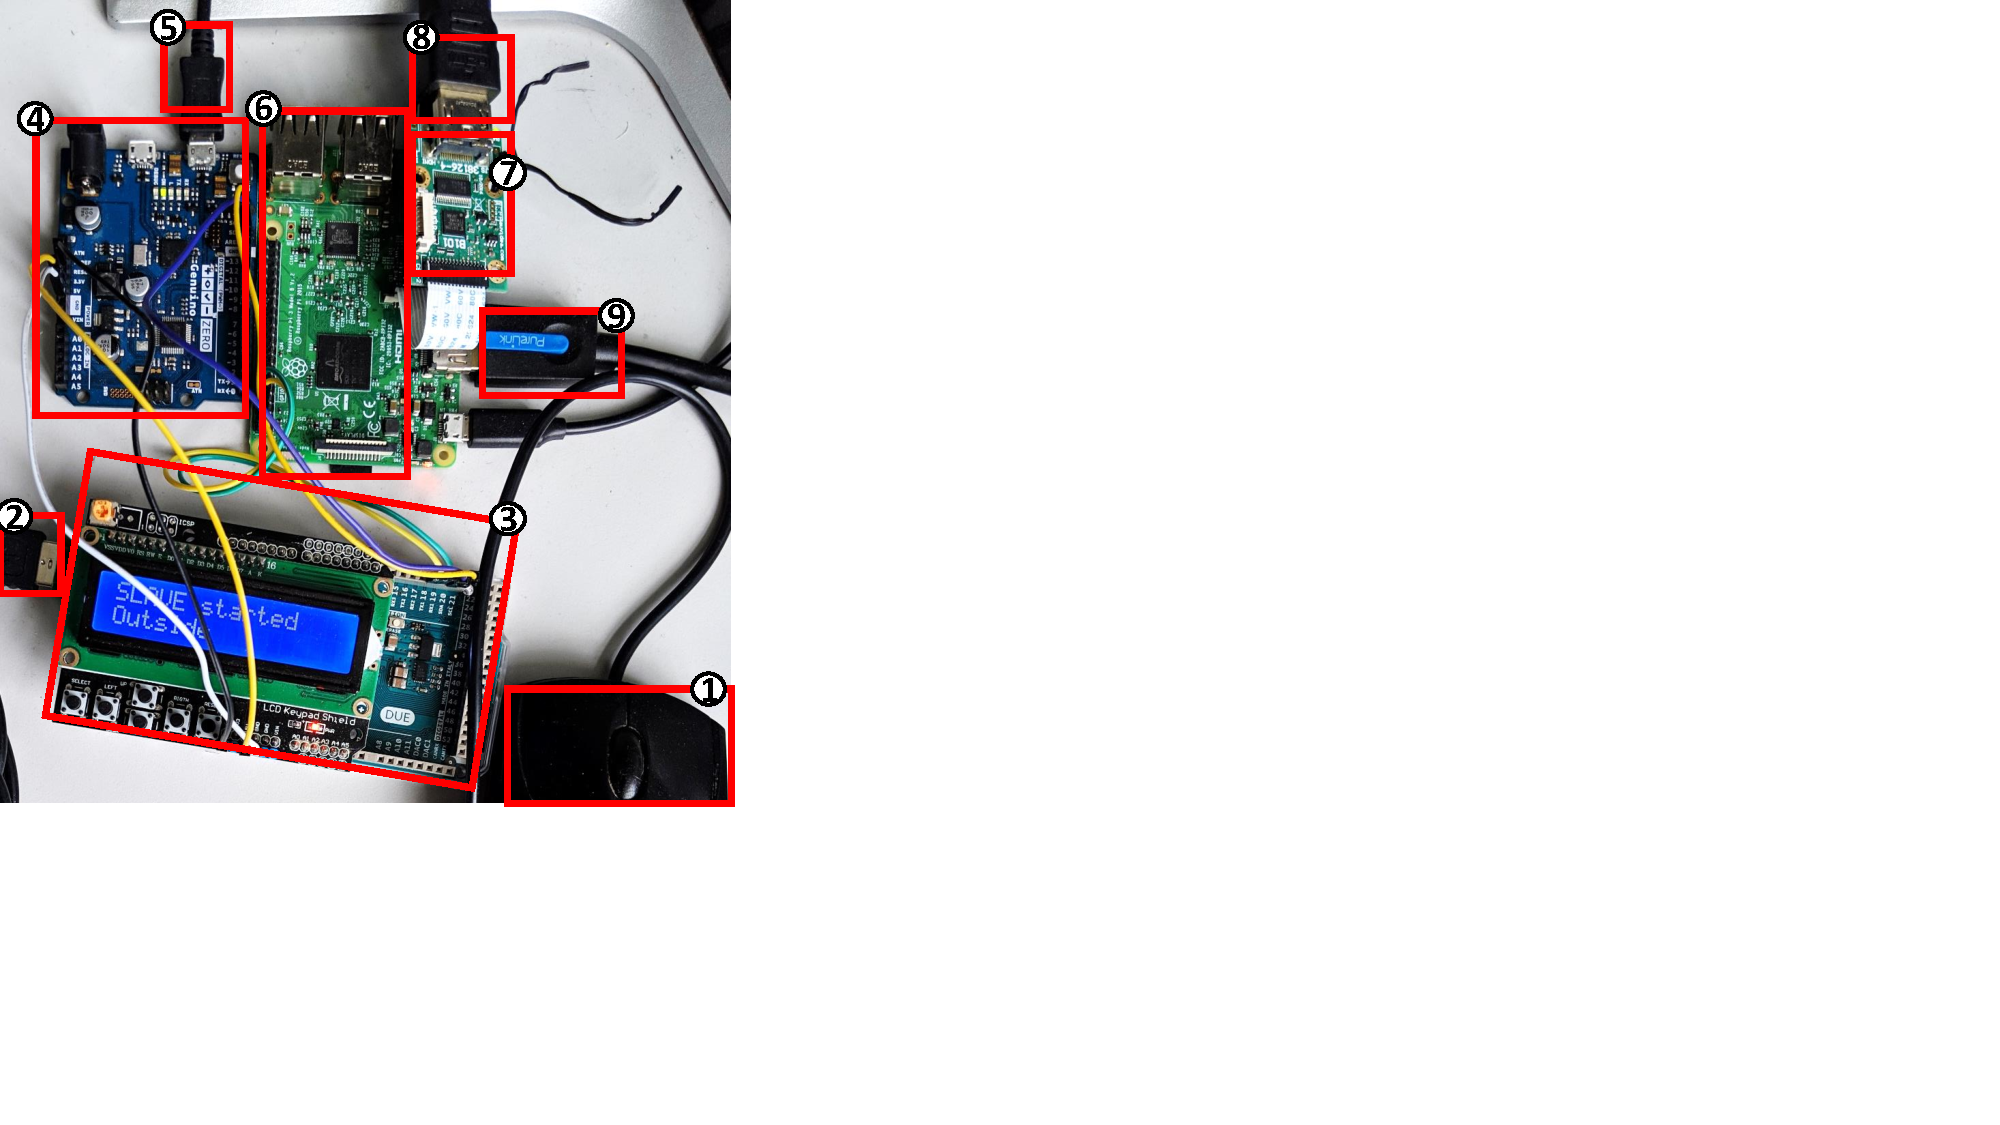
\includegraphics[trim={0 5cm 21.5cm 0}, clip, scale=0.55]{setUp_1.pdf}
		\caption{The figure shows \name prototype that employs Arduino Due and Zero microcontroller board and a Raspberry Pi 3 SBC. The highlighted numbers correspond to the labels in Figure~\ref{fig:prototypeArch}.}
		\label{fig:prototype}
	\end{subfigure}
	\end{center}
	\vspace{-1em}
	\caption{\textbf{\name prototype}. Figure~\ref{fig:prototypeArch} and~\ref{fig:prototype} shows the component diagram and a photo of the actual \name prototype respectively.} 
	\spacesave
\end{figure}


\iffalse
\begin{figure}[t]
\centering
%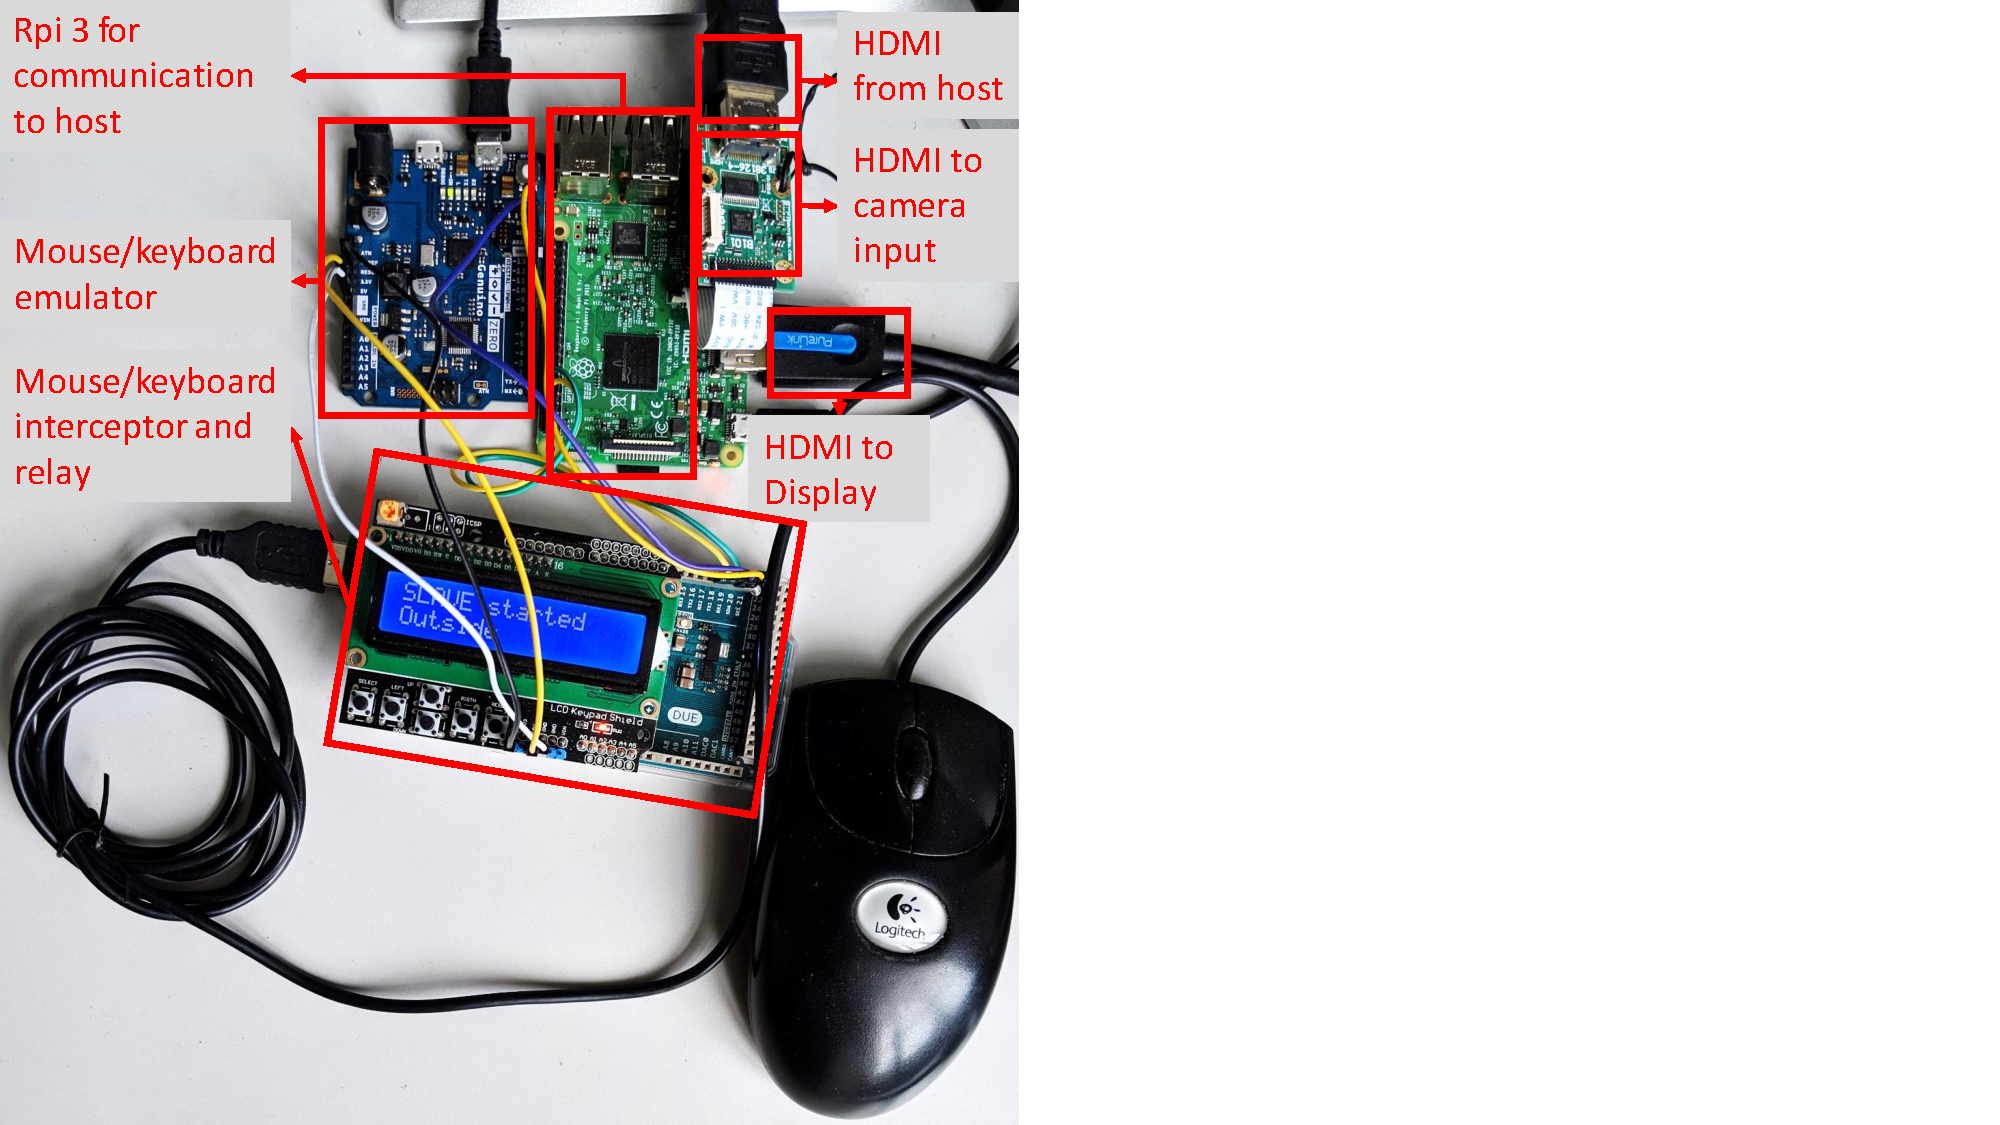
\includegraphics[trim={0 0 15cm 0}, clip, width=\linewidth]{setUp.pdf}
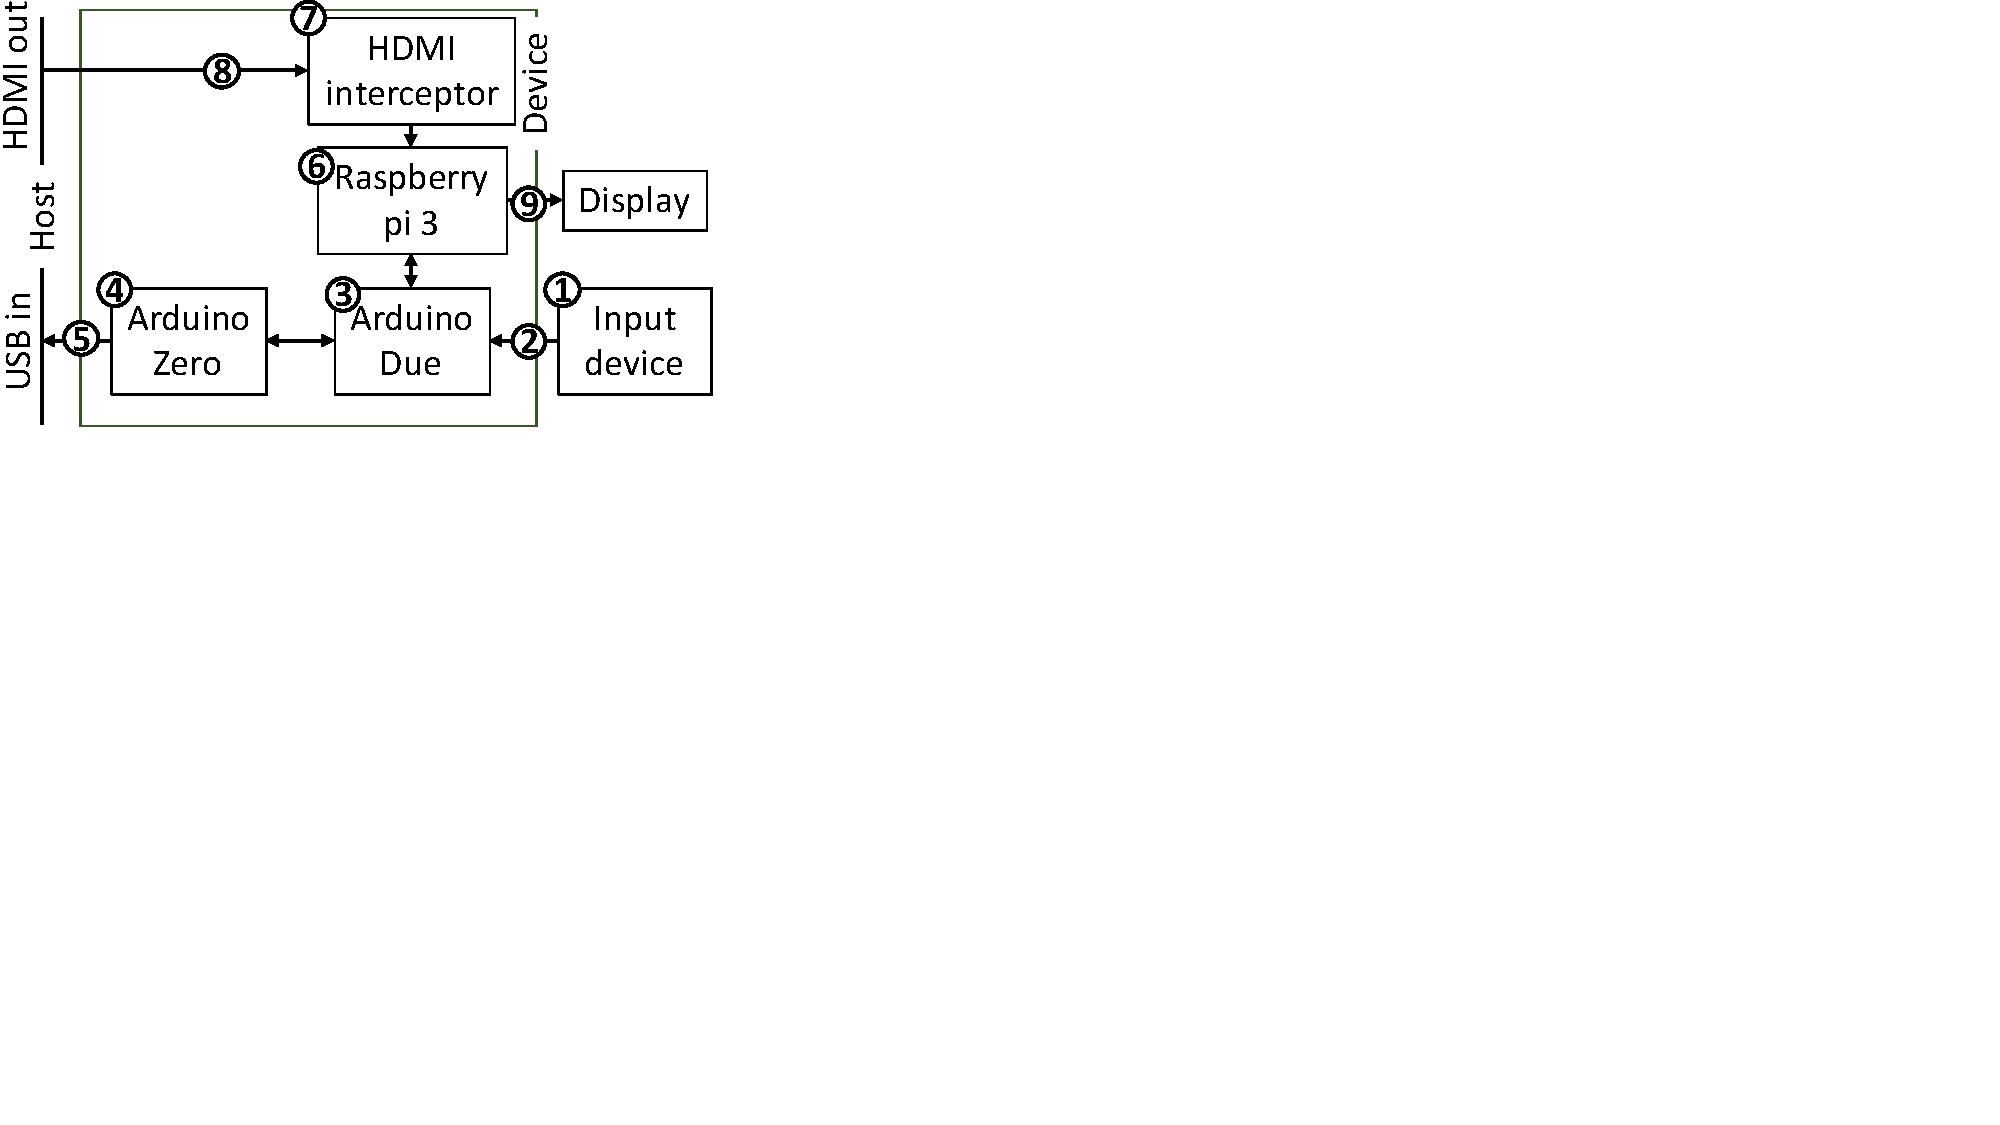
\includegraphics[trim={0 12cm 21.7cm 0}, clip, width=0.65\linewidth]{setUpBlock.pdf}
\caption{\textbf{\name prototype architecture}. }
\label{fig:prototypeArch}
\centering
\end{figure}


\begin{figure}[t]
\centering
%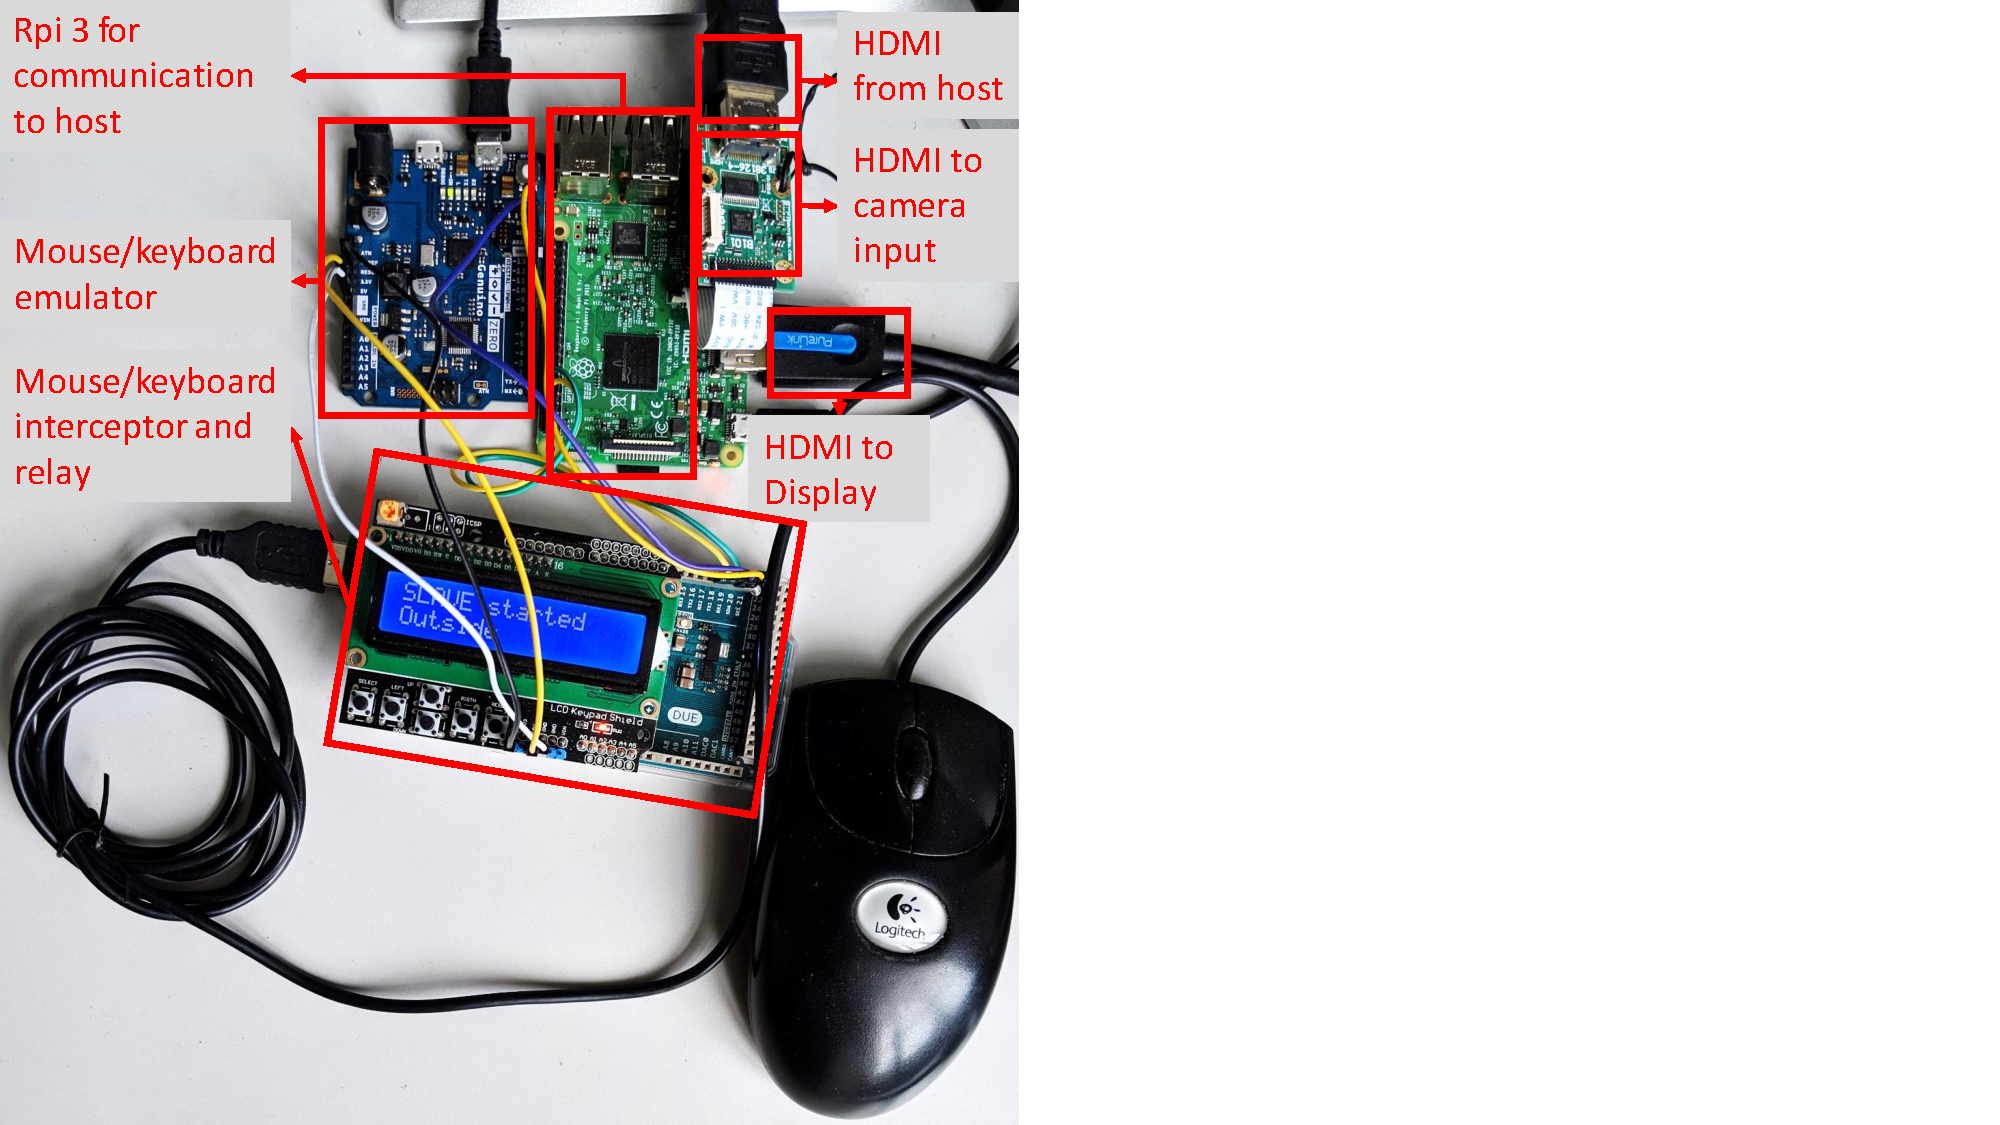
\includegraphics[trim={0 0 15cm 0}, clip, width=\linewidth]{setUp.pdf}
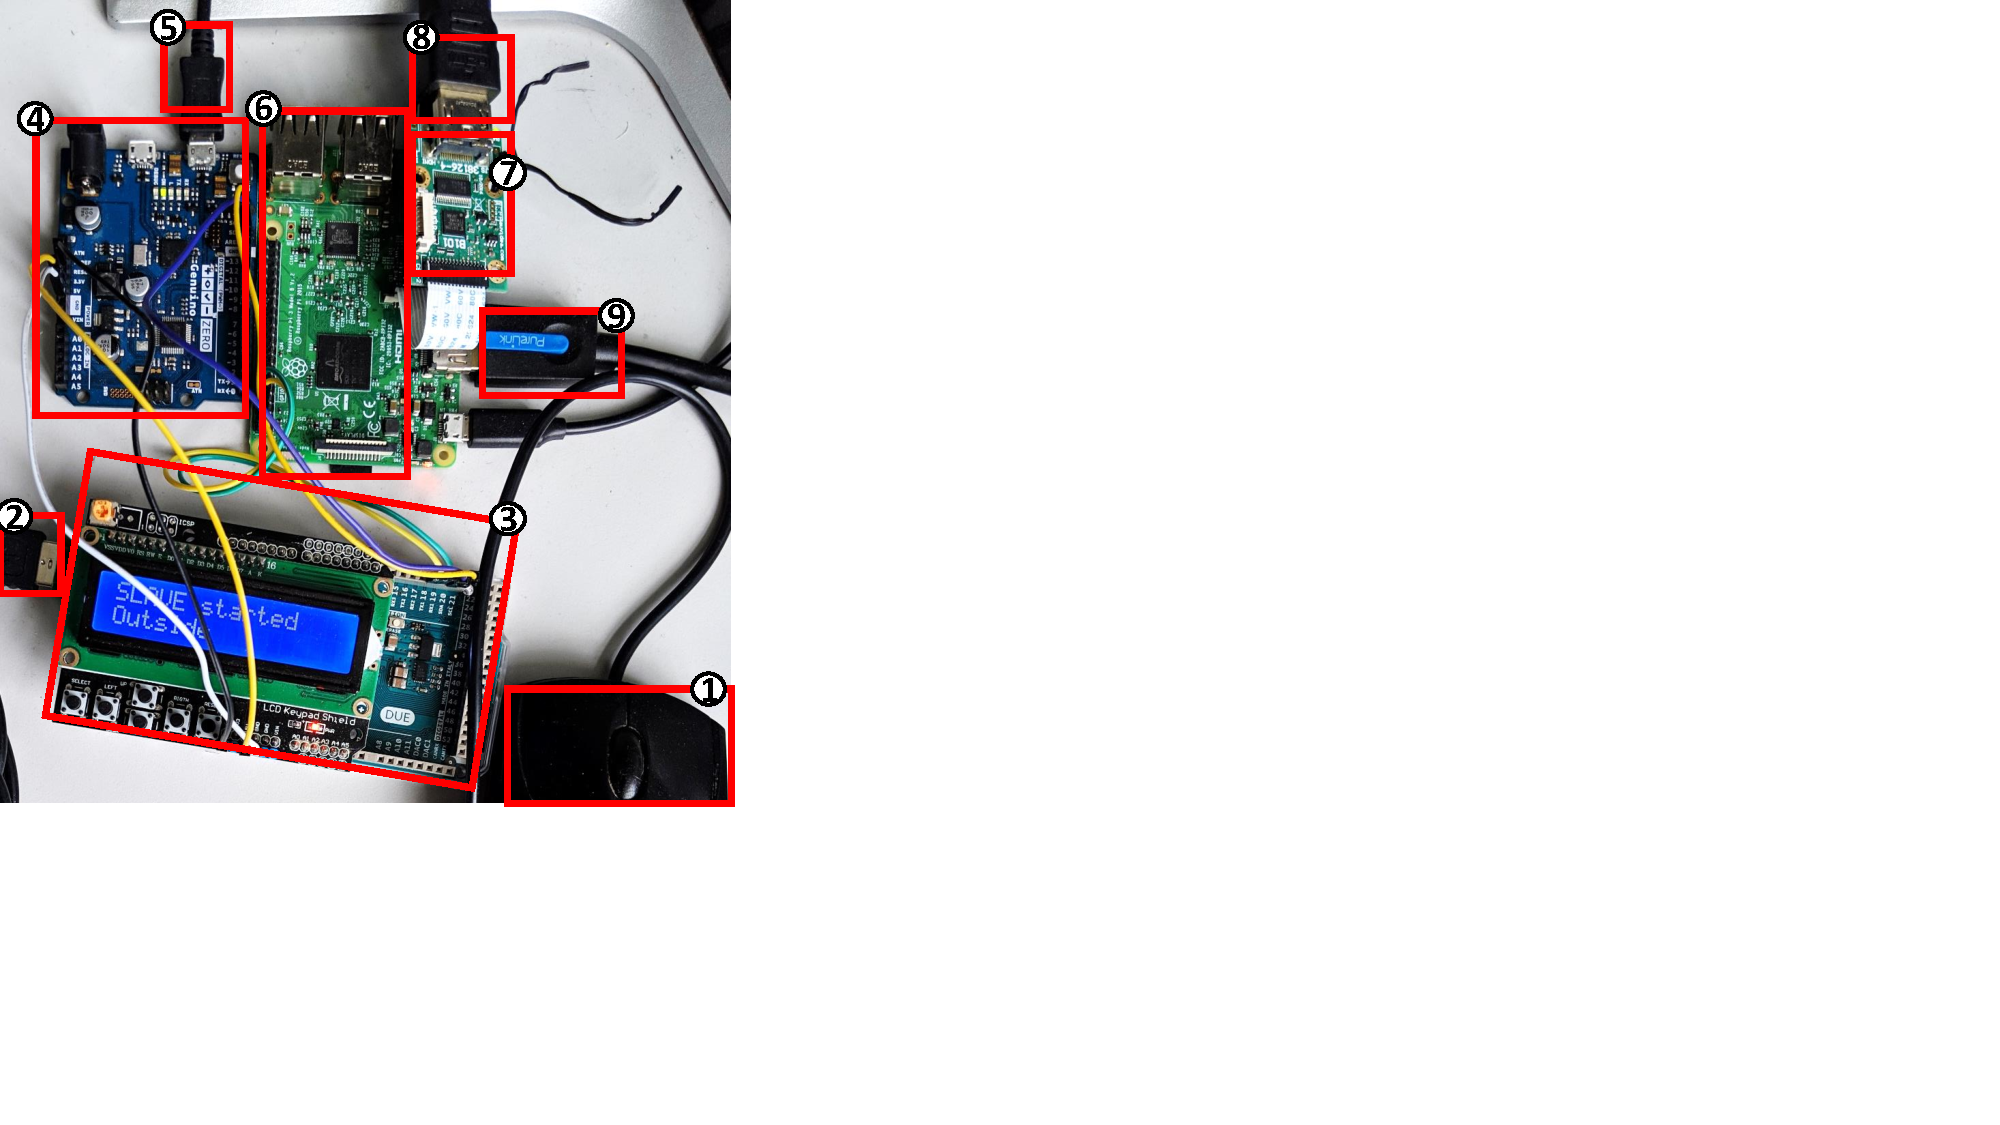
\includegraphics[trim={0 5cm 21.5cm 0}, clip, width=0.75\linewidth]{setUp_1.pdf}
\caption{\textbf{\name prototype}. The figure shows \name prototype that employs Arduino Due and Zero microcontroller board and a Raspberry Pi 3 SBC. The highlighted numbers correspond to the labels in Figure~\ref{fig:prototypeArch}.}
\spacesave
\label{fig:prototype}
\centering
\end{figure}
\fi


In this section, we describe our prototype implementation of \name as an auxiliary device. Figure~\ref{fig:prototype} depicts the \name prototype. The prototype \device is connoted to a desktop computer with 3.40 GHz Intel Core i7-6700 processor with 8 GB RAM running Ubuntu 18.04.2 LTS. The \device uses off-the-shelf components that has the following components and interfaces:

\begin{mylist}

  \item \textbf{Input interceptor.} The input interceptor is composed of a Arduino Due (\three) and an Arduino Zero (\four) that is connected to the input device over \usb (\two) interface. The input interceptor has a \usb out interface that connects to the host (\five) that relays all the user inputs to the host. 

  \item \textbf{HDMI interceptor.} The HDMI interceptor (\seven) is implemented using a B101 HDMI to CSI-2 Bridge~\cite{b101} that takes the HDMI channel (\eight) from the host and convert it to camera input signal to the Raspberry Pi 3.  
  
      \item \textbf{Compute component.} We use a Raspberry Pi 3 to implement the compute device that executes all the \device logic that includes analyzing the HDMI frame, composing the overlays, executing \tls protocol etc. Once could use an ASIC to further improve performance and reduce the code base of the compute component. The compute device is connected to the display over HDMI (\nine) interface. The compute component is implemented using Python and Java.
\end{mylist}


\subsection{Implementation of \name Components}
\label{sec:prototype:impl}


\myparagraph{Our realization of \name} \name in principle can work with generic host and application. In our prototype of \name, we implement a version of \name that works with web applications running on the browser. Our implementation of \name is realized by a low-TCB auxiliary device that acts as a hub for all IO devices. This also eliminates any need for additional software that acts as a communication channel between the \device and the host. The server and the \device communicate with QR codes (as the example screenshot shown in Figure~\ref{fig:screenshot_1}). We use QR code a a mean of a communication as it does not require any additional software to communicate and QR code is very efficient to decode as the \device recives image frame from the host. As the host renders the QR code on the screen, the \device decodes the QR code from the HDMI channel. One such example is illustrated in Figure~\ref{fig:screenshot_1} where the server sends a QR code that encodes a sensitive input form. The \device first intercepts the HDMI frames, then decodes the QR code in that frame and overlay the decoded form on the display that can be seen only by the user. Our realization of \name achieves the goals that we mentioned in Section~\ref{sec:problemStatement:goals}. \name supports generic IO devices and provides IO integrity and confidentiality (\textbf{goal 1}).The \device is implemented using a low-TCB embedded device that minimizes trust assumption (\textbf{goal 2}) and the \device is plug-and-play and requires minimum user habituation (\textbf{goal 3}). In the following, we provide the implementation details of the \name components.


\lstset{language=JSON, frame=tb, caption=\small{\textbf{Protected UI specification language.} The UI specification shows the JSON formatted UI specification that is encoded into a QR code. The specification is generated from the \html source that are tagged as protected from the developers. The example specification is generated from the \html source that is provided in corresponding UI in Figure~\ref{fig:transformation}.}, label=snippet:UISpecification, firstnumber =1}

\begin{figure}[t]
\begin{lstlisting}[mathescape=true]
{ "formId": "form1",
  "formName": "form1",
  "domain": "secure_site.io",
  "dim": "400*400",
  "SAS": "ctrl+d:5",
  "ui": [{"id":"textbox_1",
  	"type":"textbox",
	"label":"Sensitive field 1",
	"text":"secret data 1",
	"size": 40},
	{"id":"textbox_2",
	"type":"textbox",
	"label":"Sensitive field2 ",
	"text":"secret data 2",
	"size": 40},
	{"id":"b1",
	"type":"button",
	"label":"OK",
	"trigger":"true",
	"size": 10},	
	{"id":"b2",
	"type":"button",
	"label":"Cancel",
	"trigger":"true",
	"size": 10}],
  "signature": "0x45565AB246..."}
\end{lstlisting}
\end{figure}

\subsubsection{\bfseries QR code generation \& UI specification}
\label{sec:prototype:impl:qr}

QR code generation phase is executed by \name JS that transforms the UI elements of a sensitive web form to a UI specification encoded in a QR code\footnote{In the prototype implementation on \name; we use QRCode.js, a \js library to produce QR codes}. 
Section~\ref{sec:systemDesign:transformation} provides the high-level concept of generating the QR code from the webpage UI elements. UI elements that require IO integrity protection can be marked by the developers in the \html source. As illustrated in Figure~\ref{fig:transformation}, the \html UI elements: `\texttt{Sensitive field 1}' and `\texttt{Sensitive field 2}' additional attribute \texttt{protect=``true''} (one concrete example is illustrated in Figure~\ref{fig:transformation}). The \name JS iterate through all the HTML elements that have \texttt{protect=``true''} attribute. The JS then parses the HTML code and extracts information such as name of the label or type of UI element. \device uses preloaded size parameters to specify the size of a text field, button etc. in case the size is not explicitly mentioned in the HTML source. One important attribute for a UI element in the specification is the \texttt{trigger}. For example, in Specification~\ref{snippet:UISpecification}, the \texttt{OK} and the \texttt{cancel} buttons have an attribute \texttt{trigger}. This attribute is Boolean can be either \texttt{true} (corresponding to \texttt{OK}) or \texttt{false} (corresponding to \texttt{Cancel}) value. The value \texttt{true} denotes that the \texttt{OK} button can submit the values that are provided by the user. The \texttt{false} attribute denotes that hitting the \texttt{cancel} button abort the form altogether.
The QR code generation phase is between \one and \two in Figure~\ref{fig:transformation} where the \name JavaScript snippet transforms the UI elements to a UI specification language in a QR code that can be interpreted by the \device. The UI specification corresponding to the \html source (in Figure~\ref{fig:transformation}) is provided in Specification~\ref{snippet:UISpecification}. Note that the specification is highly flexible, allowing adjustable size for the form, individual UI elements, gaps between them etc. This allows the \device to faithfully recreate the UI that is very close to the actual form UI that the served by the web severer. Such allows negligible user habituation. 

\subsubsection{\bfseries Bitmap generation}

The \device reads the QR code from the HDMI frame and generate the UI overlay bitmap from it. We have used piCamera library to intercept the HDMI frames and generate the UI on top of it. 

\subsubsection{\bfseries Detection of mouse pointer}
%The \device tracks continuously the mouse pointer generated by the host and overlays its image to make the pointer prominent to the user. 
Initially, when the system boots up the \device performs the \texttt{calibration phase} (see Section \ref{pointerCalibration}) in order to synchronize its coordinates of the pointer with the host. After the calibration phase, the \device updates its mouse coordinates when a displacement event $(\Delta x_i, \Delta y_i)$ is reported by the mouse. To guarantee that the \device and the host interpret displacement events likewise, the \device performs an adjustment operation. This operation consists on the \device detecting the exact position of the host pointer in the HDMI frame by analyzing a small square of the frame (50 x 50px) around its pointer coordinates. Considering that the \device gets raw HDMI frames and pointer images are static, we use the lightweight \texttt{template matching} algorithm of the OpenCV library for the detection.

